\documentclass[tikz,border=2pt]{standalone}
\usepackage{fontspec}
\setmainfont{texgyreheros}[Extension=.otf,UprightFont=*-regular,BoldFont=*-bold,ItalicFont=*-italic]
\renewcommand{\familydefault}{\rmdefault}
\usepackage{amsmath}
\usetikzlibrary{arrows.meta,calc,positioning}
\begin{document}
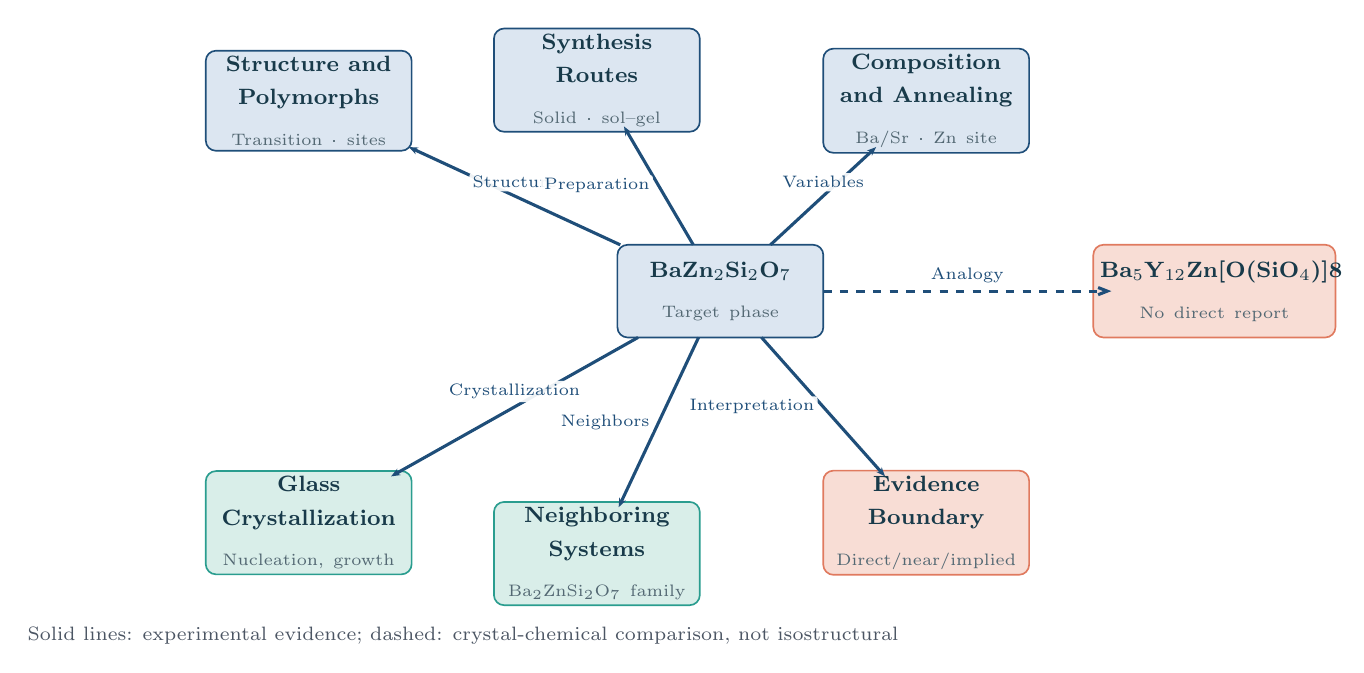
\begin{tikzpicture}[x=1pt,y=1pt, every node/.style={inner sep=0pt}]
\definecolor{nf}{HTML}{DCE6F1}\definecolor{ns}{HTML}{1f4e79}
\definecolor{lc}{HTML}{183A4A}\definecolor{sc}{HTML}{536873}
\node[draw=ns, fill=nf, line width=0.60pt, rounded corners=3.7pt, minimum width=74.4pt, minimum height=33.5pt, text width=69.4pt, align=center, inner sep=2pt, anchor=center, text opacity=0] at (223.13pt,141.32pt) {\hyphenpenalty=9000\exhyphenpenalty=9000\relax {\bfseries\fontsize{8.5}{10.1}\selectfont\color{lc}BaZn$_{2}$Si$_{2}$O$_{7}$}\\[2.6pt]{\fontsize{6.1}{7.4}\selectfont\color{sc}Target phase}};
\definecolor{nf}{HTML}{DCE6F1}\definecolor{ns}{HTML}{1f4e79}
\definecolor{lc}{HTML}{183A4A}\definecolor{sc}{HTML}{536873}
\node[draw=ns, fill=nf, line width=0.60pt, rounded corners=3.7pt, minimum width=74.4pt, minimum height=33.5pt, text width=69.4pt, align=center, inner sep=2pt, anchor=center, text opacity=0] at (74.38pt,210.12pt) {\hyphenpenalty=9000\exhyphenpenalty=9000\relax {\bfseries\fontsize{8.5}{10.1}\selectfont\color{lc}Structure and Polymorphs}\\[2.6pt]{\fontsize{6.1}{7.4}\selectfont\color{sc}Transition · sites}};
\definecolor{nf}{HTML}{DCE6F1}\definecolor{ns}{HTML}{1f4e79}
\definecolor{lc}{HTML}{183A4A}\definecolor{sc}{HTML}{536873}
\node[draw=ns, fill=nf, line width=0.60pt, rounded corners=3.7pt, minimum width=74.4pt, minimum height=33.5pt, text width=69.4pt, align=center, inner sep=2pt, anchor=center, text opacity=0] at (178.51pt,217.56pt) {\hyphenpenalty=9000\exhyphenpenalty=9000\relax {\bfseries\fontsize{8.5}{10.1}\selectfont\color{lc}Synthesis Routes}\\[2.6pt]{\fontsize{6.1}{7.4}\selectfont\color{sc}Solid · sol--gel}};
\definecolor{nf}{HTML}{DCE6F1}\definecolor{ns}{HTML}{1f4e79}
\definecolor{lc}{HTML}{183A4A}\definecolor{sc}{HTML}{536873}
\node[draw=ns, fill=nf, line width=0.60pt, rounded corners=3.7pt, minimum width=74.4pt, minimum height=33.5pt, text width=69.4pt, align=center, inner sep=2pt, anchor=center, text opacity=0] at (297.51pt,210.12pt) {\hyphenpenalty=9000\exhyphenpenalty=9000\relax {\bfseries\fontsize{8.5}{10.1}\selectfont\color{lc}Composition and Annealing}\\[2.6pt]{\fontsize{6.1}{7.4}\selectfont\color{sc}Ba/Sr · Zn site}};
\definecolor{nf}{HTML}{D9EEE9}\definecolor{ns}{HTML}{2a9d8f}
\definecolor{lc}{HTML}{183A4A}\definecolor{sc}{HTML}{536873}
\node[draw=ns, fill=nf, line width=0.60pt, rounded corners=3.7pt, minimum width=74.4pt, minimum height=33.5pt, text width=69.4pt, align=center, inner sep=2pt, anchor=center, text opacity=0] at (74.38pt,57.64pt) {\hyphenpenalty=9000\exhyphenpenalty=9000\relax {\bfseries\fontsize{8.5}{10.1}\selectfont\color{lc}Glass Crystallization}\\[2.6pt]{\fontsize{6.1}{7.4}\selectfont\color{sc}Nucleation, growth}};
\definecolor{nf}{HTML}{D9EEE9}\definecolor{ns}{HTML}{2a9d8f}
\definecolor{lc}{HTML}{183A4A}\definecolor{sc}{HTML}{536873}
\node[draw=ns, fill=nf, line width=0.60pt, rounded corners=3.7pt, minimum width=74.4pt, minimum height=33.5pt, text width=69.4pt, align=center, inner sep=2pt, anchor=center, text opacity=0] at (178.51pt,46.49pt) {\hyphenpenalty=9000\exhyphenpenalty=9000\relax {\bfseries\fontsize{8.5}{10.1}\selectfont\color{lc}Neighboring Systems}\\[2.6pt]{\fontsize{6.1}{7.4}\selectfont\color{sc}Ba$_{2}$ZnSi$_{2}$O$_{7}$ family}};
\definecolor{nf}{HTML}{F8DDD5}\definecolor{ns}{HTML}{e07a5f}
\definecolor{lc}{HTML}{183A4A}\definecolor{sc}{HTML}{536873}
\node[draw=ns, fill=nf, line width=0.60pt, rounded corners=3.7pt, minimum width=74.4pt, minimum height=33.5pt, text width=69.4pt, align=center, inner sep=2pt, anchor=center, text opacity=0] at (297.51pt,57.64pt) {\hyphenpenalty=9000\exhyphenpenalty=9000\relax {\bfseries\fontsize{8.5}{10.1}\selectfont\color{lc}Evidence Boundary}\\[2.6pt]{\fontsize{6.1}{7.4}\selectfont\color{sc}Direct/near/implied}};
\definecolor{nf}{HTML}{F8DDD5}\definecolor{ns}{HTML}{e07a5f}
\definecolor{lc}{HTML}{183A4A}\definecolor{sc}{HTML}{536873}
\node[draw=ns, fill=nf, line width=0.60pt, rounded corners=3.7pt, minimum width=87.5pt, minimum height=33.5pt, text width=82.5pt, align=center, inner sep=2pt, anchor=center, text opacity=0] at (401.64pt,141.32pt) {\hyphenpenalty=9000\exhyphenpenalty=9000\relax {\bfseries\fontsize{8.5}{10.1}\selectfont\color{lc}Ba$_{5}$Y$_{12}$Zn[O(SiO$_{4}$)]8}\\[2.6pt]{\fontsize{6.1}{7.4}\selectfont\color{sc}No direct report}};
\definecolor{ec}{HTML}{1f4e79}
\draw[draw=ec, line width=1.12pt, -{Stealth[length=3.3pt,width=2.6pt]}, rounded corners=2.2pt] (186.95pt,158.05pt) -- (110.56pt,193.38pt);
\node[fill=white, fill opacity=0.92, text opacity=1, inner sep=1.2pt, rounded corners=1pt, font=\fontsize{6.0}{6.7}\selectfont, text=ec, anchor=south, align=center] at (148.76pt,177.21pt) {Structure};
\definecolor{ec}{HTML}{1f4e79}
\draw[draw=ec, line width=1.12pt, -{Stealth[length=3.3pt,width=2.6pt]}, rounded corners=2.2pt] (213.34pt,158.05pt) -- (188.30pt,200.82pt);
\node[fill=white, fill opacity=0.92, text opacity=1, inner sep=1.2pt, rounded corners=1pt, font=\fontsize{6.0}{6.7}\selectfont, text=ec, anchor=east, align=center] at (198.96pt,179.44pt) {Preparation};
\definecolor{ec}{HTML}{1f4e79}
\draw[draw=ec, line width=1.12pt, -{Stealth[length=3.3pt,width=2.6pt]}, rounded corners=2.2pt] (241.23pt,158.05pt) -- (279.42pt,193.38pt);
\node[fill=white, fill opacity=0.92, text opacity=1, inner sep=1.2pt, rounded corners=1pt, font=\fontsize{6.0}{6.7}\selectfont, text=ec, anchor=south, align=center] at (260.32pt,177.21pt) {Variables};
\definecolor{ec}{HTML}{1f4e79}
\draw[draw=ec, line width=1.12pt, -{Stealth[length=3.3pt,width=2.6pt]}, rounded corners=2.2pt] (193.38pt,124.58pt) -- (104.13pt,74.38pt);
\node[fill=white, fill opacity=0.92, text opacity=1, inner sep=1.2pt, rounded corners=1pt, font=\fontsize{6.0}{6.7}\selectfont, text=ec, anchor=south, align=center] at (148.76pt,100.97pt) {Crystallization};
\definecolor{ec}{HTML}{1f4e79}
\draw[draw=ec, line width=1.12pt, -{Stealth[length=3.3pt,width=2.6pt]}, rounded corners=2.2pt] (215.26pt,124.58pt) -- (186.38pt,63.22pt);
\node[fill=white, fill opacity=0.92, text opacity=1, inner sep=1.2pt, rounded corners=1pt, font=\fontsize{6.0}{6.7}\selectfont, text=ec, anchor=east, align=center] at (198.96pt,93.90pt) {Neighbors};
\definecolor{ec}{HTML}{1f4e79}
\draw[draw=ec, line width=1.12pt, -{Stealth[length=3.3pt,width=2.6pt]}, rounded corners=2.2pt] (238.01pt,124.58pt) -- (282.64pt,74.38pt);
\node[fill=white, fill opacity=0.92, text opacity=1, inner sep=1.2pt, rounded corners=1pt, font=\fontsize{6.0}{6.7}\selectfont, text=ec, anchor=east, align=center] at (258.46pt,99.48pt) {Interpretation};
\definecolor{ec}{HTML}{1f4e79}
\draw[draw=ec, line width=1.12pt, -{Straight Barb[length=3.3pt,width=2.6pt]}, dashed, rounded corners=2.2pt] (260.32pt,141.32pt) -- (364.45pt,141.32pt);
\node[fill=white, fill opacity=0.92, text opacity=1, inner sep=1.2pt, rounded corners=1pt, font=\fontsize{6.0}{6.7}\selectfont, text=ec, anchor=south, align=center] at (312.39pt,142.81pt) {Analogy};
\definecolor{lc}{HTML}{183A4A}\definecolor{sc}{HTML}{536873}
\node[minimum width=74.4pt, minimum height=33.5pt, text width=69.4pt, align=center, inner sep=2pt, anchor=center] at (223.13pt,141.32pt) {\hyphenpenalty=9000\exhyphenpenalty=9000\relax {\bfseries\fontsize{8.5}{10.1}\selectfont\color{lc}BaZn$_{2}$Si$_{2}$O$_{7}$}\\[2.6pt]{\fontsize{6.1}{7.4}\selectfont\color{sc}Target phase}};
\definecolor{lc}{HTML}{183A4A}\definecolor{sc}{HTML}{536873}
\node[minimum width=74.4pt, minimum height=33.5pt, text width=69.4pt, align=center, inner sep=2pt, anchor=center] at (74.38pt,210.12pt) {\hyphenpenalty=9000\exhyphenpenalty=9000\relax {\bfseries\fontsize{8.5}{10.1}\selectfont\color{lc}Structure and Polymorphs}\\[2.6pt]{\fontsize{6.1}{7.4}\selectfont\color{sc}Transition · sites}};
\definecolor{lc}{HTML}{183A4A}\definecolor{sc}{HTML}{536873}
\node[minimum width=74.4pt, minimum height=33.5pt, text width=69.4pt, align=center, inner sep=2pt, anchor=center] at (178.51pt,217.56pt) {\hyphenpenalty=9000\exhyphenpenalty=9000\relax {\bfseries\fontsize{8.5}{10.1}\selectfont\color{lc}Synthesis Routes}\\[2.6pt]{\fontsize{6.1}{7.4}\selectfont\color{sc}Solid · sol--gel}};
\definecolor{lc}{HTML}{183A4A}\definecolor{sc}{HTML}{536873}
\node[minimum width=74.4pt, minimum height=33.5pt, text width=69.4pt, align=center, inner sep=2pt, anchor=center] at (297.51pt,210.12pt) {\hyphenpenalty=9000\exhyphenpenalty=9000\relax {\bfseries\fontsize{8.5}{10.1}\selectfont\color{lc}Composition and Annealing}\\[2.6pt]{\fontsize{6.1}{7.4}\selectfont\color{sc}Ba/Sr · Zn site}};
\definecolor{lc}{HTML}{183A4A}\definecolor{sc}{HTML}{536873}
\node[minimum width=74.4pt, minimum height=33.5pt, text width=69.4pt, align=center, inner sep=2pt, anchor=center] at (74.38pt,57.64pt) {\hyphenpenalty=9000\exhyphenpenalty=9000\relax {\bfseries\fontsize{8.5}{10.1}\selectfont\color{lc}Glass Crystallization}\\[2.6pt]{\fontsize{6.1}{7.4}\selectfont\color{sc}Nucleation, growth}};
\definecolor{lc}{HTML}{183A4A}\definecolor{sc}{HTML}{536873}
\node[minimum width=74.4pt, minimum height=33.5pt, text width=69.4pt, align=center, inner sep=2pt, anchor=center] at (178.51pt,46.49pt) {\hyphenpenalty=9000\exhyphenpenalty=9000\relax {\bfseries\fontsize{8.5}{10.1}\selectfont\color{lc}Neighboring Systems}\\[2.6pt]{\fontsize{6.1}{7.4}\selectfont\color{sc}Ba$_{2}$ZnSi$_{2}$O$_{7}$ family}};
\definecolor{lc}{HTML}{183A4A}\definecolor{sc}{HTML}{536873}
\node[minimum width=74.4pt, minimum height=33.5pt, text width=69.4pt, align=center, inner sep=2pt, anchor=center] at (297.51pt,57.64pt) {\hyphenpenalty=9000\exhyphenpenalty=9000\relax {\bfseries\fontsize{8.5}{10.1}\selectfont\color{lc}Evidence Boundary}\\[2.6pt]{\fontsize{6.1}{7.4}\selectfont\color{sc}Direct/near/implied}};
\definecolor{lc}{HTML}{183A4A}\definecolor{sc}{HTML}{536873}
\node[minimum width=87.5pt, minimum height=33.5pt, text width=82.5pt, align=center, inner sep=2pt, anchor=center] at (401.64pt,141.32pt) {\hyphenpenalty=9000\exhyphenpenalty=9000\relax {\bfseries\fontsize{8.5}{10.1}\selectfont\color{lc}Ba$_{5}$Y$_{12}$Zn[O(SiO$_{4}$)]8}\\[2.6pt]{\fontsize{6.1}{7.4}\selectfont\color{sc}No direct report}};
\definecolor{tc}{HTML}{4b5563}
\node[anchor=center, font=\fontsize{6.8}{8.1}\selectfont, text=tc] at (130.16pt,16.74pt) {Solid lines: experimental evidence; dashed: crystal-chemical comparison, not isostructural};
\end{tikzpicture}
\end{document}